% !TEX root = guia-github.tex
\documentclass[
twoside,
%openany,
12pt,                   
]{article}
\usepackage[T1]{fontenc}
\usepackage{lmodern}
\usepackage{amsmath}
\usepackage{caption}
\usepackage[a4paper]{geometry}
\usepackage{fancyhdr}
\usepackage{parskip}
\usepackage[protrusion=true, expansion=true, nopatch=footnote]{microtype}  % Use microtype to improve readability
\usepackage{graphicx,graphics}
\usepackage{indentfirst}
\usepackage{svg}
\usepackage[spanish,es-tabla]{babel}
\usepackage{hyperref}
\usepackage{listings}
\usepackage{xcolor}

\definecolor{ps-background}{RGB}{1,36,86}      % dark blue
\definecolor{ps-foreground}{RGB}{238,237,240}   % light gray
\definecolor{ps-keyword}{RGB}{135,206,250}      % light-sky blue
\definecolor{ps-string}{RGB}{255,199,34}        % gold/yellow
\definecolor{ps-comment}{RGB}{0,255,0}          % bright green
\definecolor{ps-error}{RGB}{255,85,85}          % light red

% Monospaced font (change to Consolas if using XeLaTeX/LuaLaTeX)
\newcommand{\powershellfont}{\ttfamily}

\lstdefinestyle{powershell}{
    backgroundcolor=\color{ps-background},
    basicstyle=\powershellfont\small\color{ps-foreground},
    keywordstyle=\color{ps-keyword}\bfseries,
    stringstyle=\color{ps-string},
    commentstyle=\color{ps-comment},
    identifierstyle=\color{ps-foreground},
    showstringspaces=false,
    numbers=none,
    breaklines=true,
    keepspaces=true,
    columns=fullflexible,
}

\captionsetup{
    labelfont={bf},
    textfont={small},   
    font=small
}

% Cambia el nombre de las figuras:
\addto\captionsspanish{\renewcommand{\figurename}{Fig}} 

\selectlanguage{spanish}

\newgeometry{top=2.5cm, bottom=2.5cm, right=2.5cm, left=2.5cm}

\setlength{\parskip}{7pt}   % Change the default value of paragraph spacing
\setlength{\parindent}{15pt}    %Change default paragraph indentation

\setlength{\headheight}{14.5pt}
\fancyhead[RO]{}        % Define the header for rigth (odd) pages
\fancyhead[LE]{}        % Define the header for left (even) pages
\fancyfoot[C]{\thepage} % Define the page number as the footer

\hypersetup{
    colorlinks=true,          % Enable colored links
    linkcolor=black,          % Color for internal links
    urlcolor=blue,            % Color para las URL's u texto que mande a URL's
    citecolor=blue            % Color para las citas (comando \cite{} o \citet{})
}

\begin{document}
{\LARGE \textbf{Guía para el uso de git y Github}}
\par GitHub es un servicio gratuito de internet que actúa como repositorio online de código. Github facilita la colaboración en proyectos donde intervienen muchas personas y resulta útil para controlar las distintas versiones del código y facilitar el trabajo simultáneo de varios desarrolladores.
\par Para poder hacer uso de Github, son necesarios dos pasos, que se describirán a continuación:

\section{Instalación de Git}
Git es un programa que funcionará localmente. Este se encarga de gestionar todos los archivos dentro del repositorio local y efectuar todas las operaciones de interés para subir los archivos al repositorio remoto, mezclar los cambios y avisa de todos los posibles conflictos.
\par Su instalación es relativamente sencilla, simplemente hay que descargar el programa de su \href{https://git-scm.com/install/}{\texttt{repositorio oficial}} y seguir las instrucciones para la instalación. Durante este proceso, el asistente de la instalación propondrá muchas opciones para la configuración. Si no se dispone de conocimiento sobre lo que cambiar las recomendaciones por defecto, es mejor no tocar nada y dejar las opciones por defecto. 
\par Una vez que tenemos el programa instalado, podremos hacer una prueba muy sencilla sobre su funcionamiento. Al escribir en la terminal:
\begin{lstlisting}[style=powershell]
    git --version
\end{lstlisting}
Podremos ver como respuesta algo del estilo:
\begin{lstlisting}[style=powershell]
    git version 2.34.1
\end{lstlisting}
Esto es un indicativo de que Git se ha instalado adecuadamente y que funciona correctamente, así que podremos proceder con el resto de pasos en estas instrucciones.

\section{Uso de GitHub}
Como ya se ha comentado antes, GitHub es un servicio de internet. Para poder acceder a este, es necesario disponer de una cuenta. A esta cuenta estarán asociados todos los repositorios de los que se será propietario y se podrá utilizar (con su dirección de correo asociada o el nombre de usuario) para que otros usuarios puedan compartir sus repositorios privados.
\par Además, se puede colaborar con GitHub en los repositorios públicos, los cuales son accesibles por todo el mundo (pero el propietario siempre tendrá la potestad de decidir qué pasa con el código del repositorio). 
\par Cuando ya se dispone de un repositorio remoto donde se busca trabajar, bien porque este se haya creado y esté vacío, o bien comenzando a colaborar con un grupo de personas, es necesario seguir unos cuantos pasos para tener la combinación git-GitHub funcionando.

\subsection*{Vinculación del usuario de GitHub a git}
Los primeros pasos que hay que seguir son indicar a git qué usuario y credenciales deberá utilizar para acceder a los repositorios remotos. Esto lo podremos hacer introduciendo en la terminal estas dos líneas:
\begin{lstlisting}[style=powershell]
    git config --global user.name "tu-usuario"
    git config --global user.email "tu@email.com"
\end{lstlisting}

Ahora, para acceder a un repositorio remoto que ya se ha creado, simplemente hay que seguir los siguientes pasos:
\begin{enumerate}
    \item En el caso de que el repositorio sea privado, solicitar permiso al dueño.
    \item Ejecutar, dentro de la carpeta donde se quiere copiar el repositorio remoto, la siguiente línea:
    \begin{lstlisting}[style=powershell]
git clone https://github.com/usuario/nombre-del-repo
    \end{lstlisting}
    Donde el link es el link del repositorio, por lo que \texttt{usuario} en este caso es el usuario dueño del repositorio.
    \item Verificar que el repositorio se ha copiado correctamente dentro de los archivos locales.
\end{enumerate}

A partir de ahora, cada vez que se busque copiar todos los cambios del repositorio remoto al local, el comando que habrá que ejecutar es:
\begin{lstlisting}[style=powershell]
    git pull
\end{lstlisting}

Que se encargará de copiar todos los cambios que se han hecho en el repositorio remoto y efectuarlos en el repositorio local. Esta es la forma de actualizar el repositorio local con el remoto y ponerse al día.
\par Con esto, toda la configuración básica de GitHub está hecha, y se puede proceder a describir con más detalle su uso.

\section*{Trabajando de forma colaborativa con Git}
Para poder aprovechar las ventajas de git, es importante comprender su funcionamiento. Git funciona utilizando el concepto de \textbf{ramas} o \textit{branches}, que permiten controlar el flujo de los cambios en el proyecto. Pero antes de esto, hay que establecer dos conceptos fundamentales: el del repositorio local y el repositorio remoto.
\par El repositorio local no es más que la carpeta del proyecto que se encuentra en el dispositivo desde el que se está trabajando, y existe uno por cada miembro que colabore en el proyecto. Esto funciona exactamente de la misma manera que cualquier conjunto de archivos y directorios en una máquina local. En principio, se conservan todas las libertades para poder crear, mover y modificar archivos. Veremos más adelante por qué es recomendable tener algún tipo de cuidado al hacer esto, pero en principio no hay ninguna limitación.
\par Por otro lado, está el repositorio remoto. Este es un lugar único en la nube donde todo el código puesto en común del proyecto vive. Sin embargo, esto no quiere decir que en el repositorio remoto solo pueda existir una versión del proyecto.
\par A medida que se vaya progresando con el desarrollo del proyecto en el repositorio local, se pueden ir guardando los cambios en el historial de versiones. Esto se puede conseguir muy fácilmente con dos líneas en la terminal:
\begin{lstlisting}[style=powershell]
    git add .
    git commit -m "indicaciones claras y concisas de los cambios"
\end{lstlisting}
Con esto hemos hecho dos cosas. En primer lugar, \texttt{git add{ }.} habrá tomado nota de todos los cambios y los habrá pasado al ``staging area'', mientras que \texttt{git commit} guardará todos los cambios del ``staging area''. Con esto, tendremos hecho un \textbf{commit} en nuestro repositorio local. Para pasar estos cambios al repositorio remoto, podemos utilizar:
\begin{lstlisting}[style=powershell]
    git push
\end{lstlisting}

Que se encargará de subir todos los \textbf{commits} nuevos al repositorio remoto. Sin embargo, esto nos deja con una posible fuente de conflictos en el caso de un desarrollo colaborativo. Si dos personas hace modificaciones en el mismo archivo en sus respectivos repositorios locales y quisieran subir ambos sus cambios al repositorio remoto, habrá conflictos. Estos surgirán en git indicando que hay varios cambios nuevos en el mismo archivo, y que no sabe cuáles son los que debe conservar (y entonces comenzará el tedioso trabajo de ir línea a línea eligiendo cuál conservar). Para evitar esto, se introduce el concepto de las ramas o \textit{branches}, como se puede ver representado en la \autoref{fig:git-branches}

\begin{figure}[ht]
    \centering
    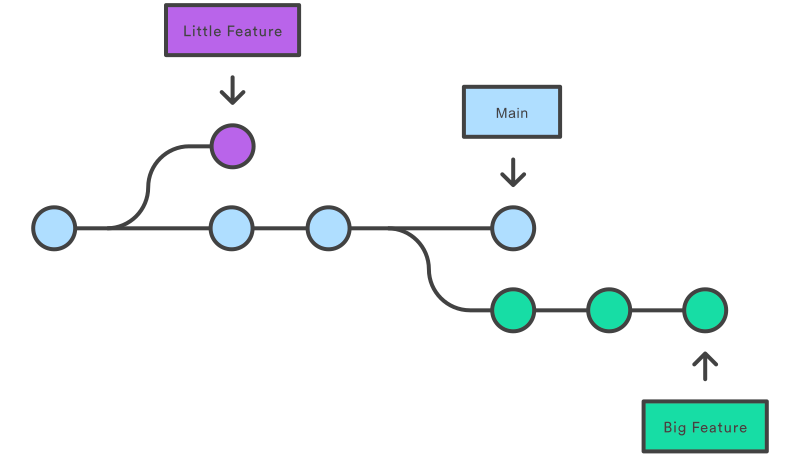
\includegraphics[width= 0.5\linewidth]{figures/git-brach.png}
    \caption{Diagrama del funcionamiento de las ramas en GitHub}\label{fig:git-branches}
\end{figure}

A la hora de añadir cualquier tipo de funcionalidad nueva al proyecto, la mejor práctica es hacer una nueva rama desde el estado anterior (normalmente la rama principal, o \textbf{main branch}) y hacer allí todos los commits que sea necesario. Cuando la funcionalidad haya sido deibdamente implementada (recomendable que se haya hecho añadiendo archivos nuevos y evitando modificar los originales en la mayor medida de lo posible), se podrá combinar esta rama con la principal.

\subsection*{Cómo abrir una rama nueva}
Cuando se estima que se van a desarrollar una serie de cambios nuevos, puede resultar interesante abrir una rama nueva para poder separar el desarrollo de estas características del de las demás. En estos casos, lo más interesante es declarar una nueva rama en el repositorio remoto y comenzar a subir los cambios allí. Los comandos para hacer esto son:
\begin{lstlisting}[style=powershell]
    git checkout -b nombre-rama
\end{lstlisting}
Con esto, habremos creado una nueva rama y estaremos trabajando en ella. Esto se podrá confirmar con \texttt{git branch}, que proporcionará una lista de las ramas disponibles en el repositorio. 
\par A medida que se progresa con el desarrollo, se continuará con el flujo de trabajo típico de:
\begin{lstlisting}[style=powershell]
    git add .
    git commit -m "descripcion de los cambios"
\end{lstlisting}
Hasta que se llegue a un hito importante, y entonces la forma de sincronizar los cambios al repositorio remoto es con:
\begin{lstlisting}[style=powershell]
    git push -u origin nombre-rama
\end{lstlisting}
Aquí, la \texttt{-u} quiere decir: ``a partir de ahora, todas los \textit{commits} que haga deben ir a la rama \texttt{nombre-rama}''. Con esto, habremos subido los cambios al repositorio remoto en la rama nueva, y los cambios que subamos serán en esta misma rama nueva. No obstante, para proyectos no muy grandes, es interesante trabajar en la rama principal. Los mismos git o GitHub se encargarán de conservar el historial de versiones y facilitarán volver atrás en caso de ``liarla'' y que surja la necesidad de revertir los cambios.

\section*{Configuración de git desde el escritorio remoto UPM}
Uno de los usos más útiles de esta herramienta, es para poder trabajar cómodamente entre varias estaciones de trabajo. Por ejemplo, FLUENT es un programa que está disponible en el escritorio UPM, y su instalación es compleja. Por otro lado, trabajar en fluent genera una grandísima cantidad de archivos y su transferencia mediante una memoria portátil (USB) o mandando el directorio de trabajo no es rápido. Para solucionar esto, la recomendación es activar git en el escritorio remoto, que viene ya instalado. 

\subsection*{Configuración previa en GitHub}
Para tener acceso al repositorio de GitHub desde una máquina cualquiera, es necesario iniciar sesión. Es muy recomendable, en lugar de iniciar sesión de la forma estándar, utilizar un \textit{token} personalizado para reducir los permisos concedidos a los estrictamente necesarios. De esta forma, se reduce el riesgo de compartir por error el \textit{token} de acceso. 
\par Para conseguir el \textit{token}, el procedimiento a seguir desde la página web de GitHub es el siguiente:
\begin{enumerate}
    \item En GitHub, haciendo click sobre el icono del perfil a la derecha, ir a ajustes $\to$ Ajustes de desarrollador (Developer settings)
    \item Personal access tokens $\to$ Fine-grained tokens $\to$ Generate new token
    \item Daremos un nombre y una descripción al token, y seleccionaremos \textbf{All repositories}.
    \item En Permissions, daremos permisos de lectura y escritura (en cada permiso) para:
    \begin{itemize}
        \vspace{-0.5em}
        \item Pull requests
        \vspace{-0.5em}
        \item Commit statuses
        \vspace{-0.5em}
        \item Contents
    \end{itemize}
    Se añadirá el permiso de metadata en read-only, es normal.
    \item Generaremos el token y en la pantalla a continuación, es muy importante copiarlo y guardarlo en un sitio seguro, ya que esta será la contraseña que siempre se debe usar para iniciar sesión en una máquina remota.
\end{enumerate}
Con el \textit{token} ya generado y disponible, podemos iniciar git en el escritorio virtual. La recomendación más cómoda para hacer esto, es abrir una terminal en el escritorio. Para ello, se puede hacer \textbf{click derecho} sobre un espacio vacío en el escritorio $\to$ abrir en terminal. En esta línea de comandos introduciremos los típicos:
\begin{lstlisting}[style=powershell]
    git init
    git config --global user.name "nombre-usuario"
    git config --global user.email "tucorreo@gmail.com"

    git clone https://github.com/nombre-usuario/nombre-repositorio
\end{lstlisting}
En este momento, nos pedirá git que iniciemos sesión para clonar el repositorio. Se seleccionará la opción de iniciar sesión mediante token, y a continuación se puede introducir el token (recomiendo copiarlo y pegarlo)
\begin{lstlisting}[style=powershell]
    cd nombre-repositorio
\end{lstlisting}
Con esta retahíla de comandos habremos:
\begin{enumerate}
    \item Iniciado git en el escritorio,
    \item Configurado el usuario y la cuenta,
    \item Hecho una copia en el escritorio del repositorio remoto, e iniciado sesión con el token de acceso personal, y
    \item Hemos cambiado el directorio de trabajo a dentro del repositorio (equivalente a abrir la consola dentro del repositorio).
\end{enumerate}
Con esto, estaremos trabajando en la rama principal del repositorio remoto, y a partir de ahora, podremos guardar los cambios con el flujo de trabajo típico de:
\begin{lstlisting}[style=powershell]
    git add .
    git commit -m "descripcion de los cambios"
    git push
\end{lstlisting}

\end{document}